\section{Optimale 1-fehlerkorrigierende Codes}



% \subsection*{Von der Kartentrick-Methode zu optimalen Codes}

Mit der Kartentrick-Methode haben wir ein Verfahren kennengelernt,
mit dem sich einzelne Bitfehler nicht nur erkennen, sondern auch
korrigieren lassen. Dazu werden die Bits einer Nachricht in einer
Tabelle angeordnet und für jede Zeile und jede Spalte Kontrollbits
ergänzt. Für eine Nachricht mit 16 Bit benötigen wir bei einer
Anordnung in einer \(4\times 4\)-Tabelle insgesamt 9 Kontrollbits.
Aus den ursprünglichen 16 Bit entsteht somit ein Codewort mit
25 Bit.

Die Kartentrick-Methode funktioniert zwar zuverlässig, benötigt
aber relativ viele zusätzliche Bits. Es stellt sich deshalb die
Frage, ob sich dieselbe Fehlerkorrektur auch mit weniger
Kontrollbits erreichen lässt.


\subsection*{Überwachungsbereiche der Kontrollbits}

Um diese Frage zu untersuchen, betrachten wir genauer, welche Bits
durch die einzelnen Kontrollbits überwacht werden. Wir bezeichnen
die ursprünglichen Nachrichtenbits mit
\(a_1,a_2,\ldots,a_{16}\) und die neun Kontrollbits mit
\(c_1,c_2,\ldots,c_9\).

Beispielsweise überwacht das Kontrollbit \(c_1\) die vier
Nachrichtenbits \(a_1,a_5,a_9,a_{13}\). Sein Wert wird so gewählt,
dass die Anzahl Einsen unter diesen fünf Bits gerade ist.

\begin{center}
    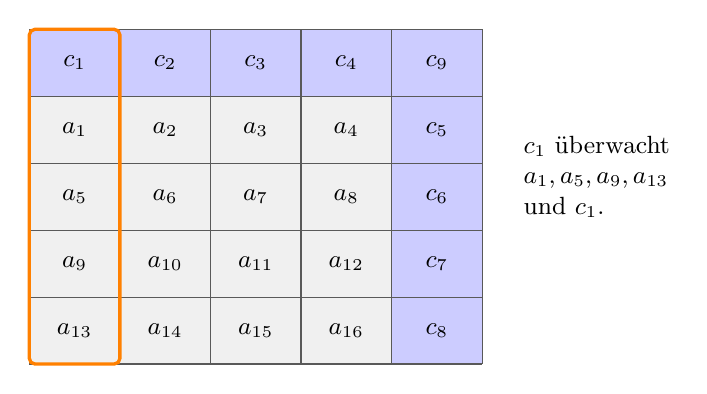
\begin{tikzpicture}[
            x=1.15cm,y=0.85cm,
            every node/.style={font=\small}
        ]
        % Nachrichtenbits
        \foreach \r in {1,...,4} {
                \foreach \c in {1,...,4} {
                        \pgfmathtruncatemacro{\nr}{4*(\r-1)+\c}
                        \fill[gray!12] (\c-1,-\r) rectangle (\c,-\r+1);
                        \node at (\c-.5,-\r+.5) {\(a_{\nr}\)};
                    }
            }

        % Kontrollbits der Spalten
        \foreach \c in {1,...,4} {
                \fill[blue!20] (\c-1,0) rectangle (\c,1);
                \node at (\c-.5,.5) {\(c_{\c}\)};
            }

        % Kontrollbits der Zeilen
        \foreach \r in {1,...,4} {
                \pgfmathtruncatemacro{\nr}{\r+4}
                \fill[blue!20] (4,-\r) rectangle (5,-\r+1);
                \node at (4.5,-\r+.5) {\(c_{\nr}\)};
            }

        % Kontrollbit oben rechts
        \fill[blue!20] (4,0) rectangle (5,1);
        \node at (4.5,.5) {\(c_9\)};

        % Gitter
        \draw[step=1,black!65] (0,-4) grid (5,1);

        % Beispiel: Überwachungsbereich von c1
        \draw[orange,very thick,rounded corners=2pt]
        (0,-4) rectangle (1,1);

        \node[anchor=west,align=left] at (5.35,-1.2)
        {\(c_1\) überwacht\\
            \(a_1,a_5,a_9,a_{13}\)\\
            und \(c_1\).};
    \end{tikzpicture}
\end{center}


Die Überwachungsbereiche lassen sich in einer sogenannten
\emph{Überwachungstabelle} darstellen. Jede Spalte entspricht
einem Bit des Codeworts und jede Zeile einem Kontrollbit.
Ein Kreuz in der Tabelle bedeutet, dass das entsprechende Bit
vom jeweiligen Kontrollbit überwacht wird.


\begin{center}
    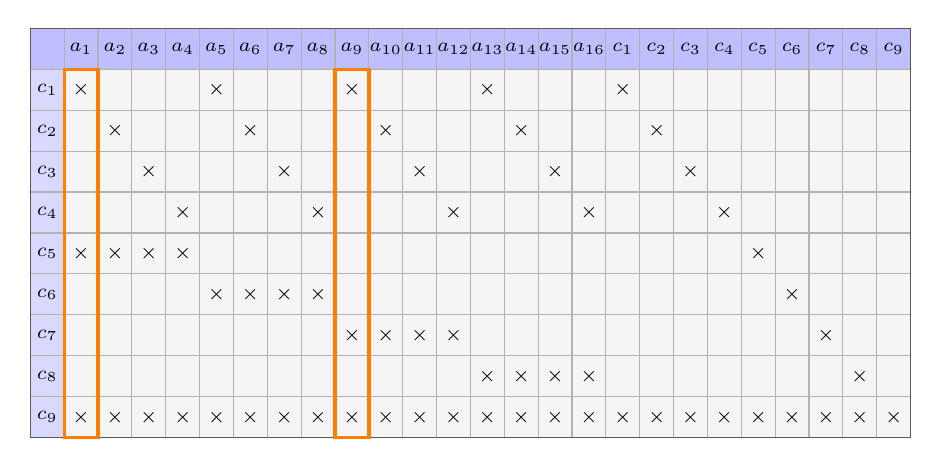
\begin{tikzpicture}[
            x=0.43cm,y=0.52cm,
            every node/.style={font=\scriptsize}
        ]
        % Tabellenhintergrund
        \fill[blue!25] (0,0) rectangle (26,1);
        \fill[blue!15] (0,-9) rectangle (1,0);
        \fill[gray!8] (1,-9) rectangle (26,0);

        % Spaltenbeschriftung
        \foreach \i in {1,...,16} {
                \pgfmathsetmacro{\xx}{\i+.5}
                \node at (\xx,.5) {\(a_{\i}\)};
            }
        \foreach \i in {1,...,9} {
                \pgfmathtruncatemacro{\col}{16+\i}
                \node at (\col+.5,.5) {\(c_{\i}\)};
            }

        % Zeilenbeschriftung
        \foreach \i in {1,...,9} {
                \node at (.5,.5-\i) {\(c_{\i}\)};
            }

        % Kontrollbits c1 bis c4 (Spalten)
        \foreach \j in {1,...,4} {
                \foreach \r in {0,...,3} {
                        \pgfmathtruncatemacro{\col}{\j+4*\r}
                        \node at (\col+.5,.5-\j) {\(\times\)};
                    }
            }

        % Kontrollbits c5 bis c8 (Zeilen)
        \foreach \r in {1,...,4} {
                \pgfmathtruncatemacro{\row}{\r+4}
                \foreach \j in {1,...,4} {
                        \pgfmathtruncatemacro{\col}{4*(\r-1)+\j}
                        \node at (\col+.5,.5-\row) {\(\times\)};
                    }
            }

        % Jedes Kontrollbit überwacht sich selbst
        \foreach \i in {1,...,8} {
                \pgfmathtruncatemacro{\col}{16+\i}
                \node at (\col+.5,.5-\i) {\(\times\)};
            }

        % c9 überwacht sämtliche Bits
        \foreach \col in {1,...,25} {
                \node at (\col+.5,-8.5) {\(\times\)};
            }

        % Gitter
        \draw[step=1,black!30,thin] (0,-9) grid (26,1);
        \draw[black!65] (0,-9) rectangle (26,1);

        % Hervorhebung der ersten Spalte
        \draw[orange,very thick]
        (1,-9) rectangle (2,0);

        % Hervorhebung der ersten Spalte
        \draw[orange,very thick]
        (9,-9) rectangle (10,0);
    \end{tikzpicture}
\end{center}


Tritt bei der Übertragung ein einzelner Bitfehler auf, so stimmen
die Paritätsbedingungen genau jener Kontrollbits nicht mehr,
die das fehlerhafte Bit überwachen. Beispielsweise wird ein Fehler
im Bit \(a_1\) von den Kontrollbits \(c_1,c_5\) und \(c_9\)
registriert. Ein Fehler im Bit \(a_9\) wird dagegen von
\(c_1,c_7\) und \(c_9\) registriert. (Markierte Spalten in der Überwachungstabelle.)

Die Kombination der Kontrollbits, die einen Fehler registrieren,
bildet somit eine Art \emph{Signatur des fehlerhaften Bits}.
Anhand dieser Signatur können wir bestimmen, welches Bit
umgeflippt wurde.

Damit dies eindeutig möglich ist, müssen die Spalten der
Überwachungstabelle paarweise verschieden sein. Ausserdem darf
keine Spalte ausschliesslich aus leeren Feldern bestehen, da
ein Fehler im entsprechenden Bit sonst von keinem Kontrollbit
erkannt würde.
\begin{myremark}
    Eine Kodierung ist genau dann 1-fehlerkorrigierend,
    wenn die Spalten ihrer Überwachungstabelle paarweise verschieden
    und keine davon leer ist.
\end{myremark}



\subsection*{Wie viele Kontrollbits sind mindestens notwendig?}

Betrachten wir nun eine Nachricht mit 16 Bit. Bei der
Kartentrick-Methode haben wir dafür neun Kontrollbits verwendet.
Allerdings zeigt die Überwachungstabelle, dass das neunte
Kontrollbit \(c_9\) überflüssig ist: Auch wenn wir auf dieses
Kontrollbit verzichten, bleiben alle Spalten paarweise
verschieden und nicht leer. Wir können also bereits mit
acht Kontrollbits sämtliche Einzelfehler korrigieren.

Doch wie viele Kontrollbits benötigen wir mindestens?

Mit \(n\) Kontrollbits besitzt die Überwachungstabelle \(n\) Zeilen.
In jeder Spalte kann ein Kreuz entweder vorhanden sein oder
fehlen. Somit gibt es insgesamt \(2^n\) verschiedene Möglichkeiten,
eine Spalte zu gestalten. Da eine Spalte ohne Kreuze nicht
verwendet werden darf, bleiben

\[
    2^n-1
\]

nutzbare Spalten.

Für eine Nachricht mit 16 Bit und \(n\) Kontrollbits benötigen
wir insgesamt \(16+n\) verschiedene Spalten. Deshalb muss gelten:

\[
    2^n-1\geq 16+n.
\]

Mit vier Kontrollbits erhalten wir höchstens
\(2^4-1=15\) nutzbare Spalten. Dies reicht nicht aus.
Mit fünf Kontrollbits stehen dagegen
\(2^5-1=31\) verschiedene Spalten zur Verfügung.
Das genügt für die insgesamt 21 Bits des Codeworts.

Für die 1-fehlerkorrigierende Kodierung einer Nachricht
mit 16 Bit sind somit mindestens fünf Kontrollbits notwendig.

\begin{myremark}
    Allgemein gilt für eine Nachricht der Länge \(m\), dass die
    minimale Anzahl \(n\) der Kontrollbits die folgende Ungleichung
    erfüllen muss:
    \[
        2^n-1\geq m+n
    \]
\end{myremark}





\subsection*{Konstruktion einer optimalen Überwachungstabelle}

Wir wissen nun, dass fünf Kontrollbits für eine Nachricht
mit 16 Bit ausreichen können. Wie lässt sich eine
entsprechende Kodierung konstruieren?

Dazu erstellen wir eine Überwachungstabelle mit fünf Zeilen
und 21 Spalten. Die ersten 16 Spalten entsprechen den
Nachrichtenbits \(a_1,\ldots,a_{16}\), die letzten fünf den
Kontrollbits \(c_1,\ldots,c_5\).

\begin{center}
    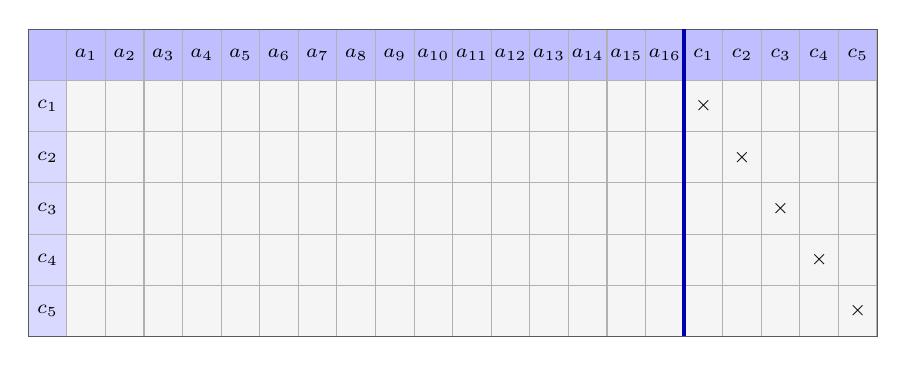
\begin{tikzpicture}[
            x=0.49cm,y=0.65cm,
            every node/.style={font=\scriptsize}
        ]
        % Hintergrund
        \fill[blue!25] (0,0) rectangle (22,1);
        \fill[blue!15] (0,-5) rectangle (1,0);
        \fill[gray!8] (1,-5) rectangle (22,0);

        % Spaltenbeschriftung
        \foreach \i in {1,...,16} {
                \node at (\i+.5,.5) {\(a_{\i}\)};
            }
        \foreach \i in {1,...,5} {
                \pgfmathtruncatemacro{\col}{16+\i}
                \node at (\col+.5,.5) {\(c_{\i}\)};
            }

        % Zeilenbeschriftung
        \foreach \i in {1,...,5} {
                \node at (.5,.5-\i) {\(c_{\i}\)};
            }

        % Überwachungsbereiche der Nachrichtenbits
        % Entsprechend der Tabelle auf Folie 13
        % \foreach \col in {1,2,3,4,11,12,13} {
        %         \node at (\col+.5,-.5) {\(\times\)};
        %     }
        % \foreach \col in {1,5,6,7,11,12,13,14,15} {
        %         \node at (\col+.5,-1.5) {\(\times\)};
        %     }
        % \foreach \col in {2,5,8,9,11,14,16} {
        %         \node at (\col+.5,-2.5) {\(\times\)};
        %     }
        % \foreach \col in {3,6,8,10,12,14,15,16} {
        %         \node at (\col+.5,-3.5) {\(\times\)};
        %     }
        % \foreach \col in {4,7,9,10,13,15,16} {
        %         \node at (\col+.5,-4.5) {\(\times\)};
        %     }

        % Kontrollbits: Einheitsmatrix
        \foreach \i in {1,...,5} {
                \pgfmathtruncatemacro{\col}{16+\i}
                \node at (\col+.5,.5-\i) {\(\times\)};
            }

        % Gitter
        \draw[step=1,black!30,thin] (0,-5) grid (22,1);
        \draw[black!65] (0,-5) rectangle (22,1);

        % Trennung Nachrichtenbits / Kontrollbits
        \draw[blue!70!black,very thick] (17,-5) -- (17,1);
    \end{tikzpicture}
\end{center}

Jedes Kontrollbit überwacht sich selbst. Daher tragen wir
in der Spalte von \(c_1\) ein Kreuz in der ersten Zeile ein,
in der Spalte von \(c_2\) eines in der zweiten Zeile usw.
Die übrigen Felder dieser fünf Spalten bleiben leer.

Die Einträge für die 16 Nachrichtenbits wählen wir
anschliessend so, dass alle Spalten paarweise verschieden
und nicht leer sind. Dabei gibt es verschiedene Möglichkeiten.
Jede solche Wahl führt zu einer 1-fehlerkorrigierenden
Kodierung mit fünf Kontrollbits.


\begin{center}
    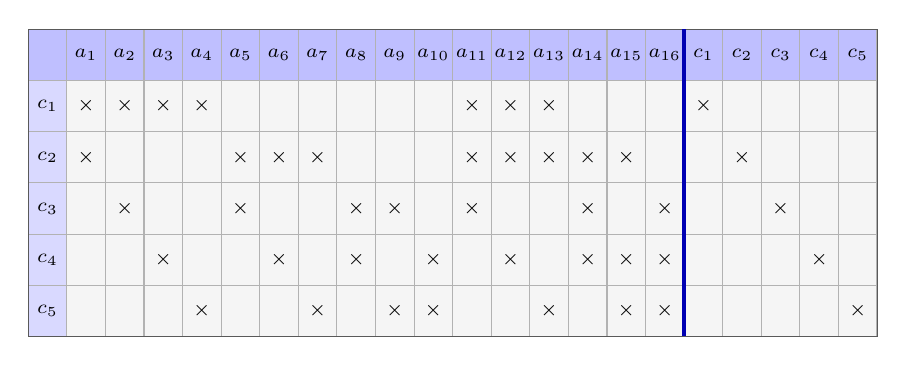
\begin{tikzpicture}[
            x=0.49cm,y=0.65cm,
            every node/.style={font=\scriptsize}
        ]
        % Hintergrund
        \fill[blue!25] (0,0) rectangle (22,1);
        \fill[blue!15] (0,-5) rectangle (1,0);
        \fill[gray!8] (1,-5) rectangle (22,0);

        % Spaltenbeschriftung
        \foreach \i in {1,...,16} {
                \node at (\i+.5,.5) {\(a_{\i}\)};
            }
        \foreach \i in {1,...,5} {
                \pgfmathtruncatemacro{\col}{16+\i}
                \node at (\col+.5,.5) {\(c_{\i}\)};
            }

        % Zeilenbeschriftung
        \foreach \i in {1,...,5} {
                \node at (.5,.5-\i) {\(c_{\i}\)};
            }

        % Überwachungsbereiche der Nachrichtenbits
        % Entsprechend der Tabelle auf Folie 13
        \foreach \col in {1,2,3,4,11,12,13} {
                \node at (\col+.5,-.5) {\(\times\)};
            }
        \foreach \col in {1,5,6,7,11,12,13,14,15} {
                \node at (\col+.5,-1.5) {\(\times\)};
            }
        \foreach \col in {2,5,8,9,11,14,16} {
                \node at (\col+.5,-2.5) {\(\times\)};
            }
        \foreach \col in {3,6,8,10,12,14,15,16} {
                \node at (\col+.5,-3.5) {\(\times\)};
            }
        \foreach \col in {4,7,9,10,13,15,16} {
                \node at (\col+.5,-4.5) {\(\times\)};
            }

        % Kontrollbits: Einheitsmatrix
        \foreach \i in {1,...,5} {
                \pgfmathtruncatemacro{\col}{16+\i}
                \node at (\col+.5,.5-\i) {\(\times\)};
            }

        % Gitter
        \draw[step=1,black!30,thin] (0,-5) grid (22,1);
        \draw[black!65] (0,-5) rectangle (22,1);

        % Trennung Nachrichtenbits / Kontrollbits
        \draw[blue!70!black,very thick] (17,-5) -- (17,1);
    \end{tikzpicture}
\end{center}


Um eine Nachricht zu kodieren, bestimmen wir die Kontrollbits
nacheinander. Dabei betrachten wir jeweils diejenigen
Nachrichtenbits, die vom entsprechenden Kontrollbit überwacht
werden. Das Kontrollbit wird so gewählt, dass die Gesamtzahl
der Einsen gerade ist.

\begin{myexample}
    Die Nachricht

    \[
        \texttt{0101 1111 0010 1011}
    \]

    soll mit der Überwachungstabelle oben durch Kontrollbits ergänzt werden.

    Das Kontrollbit \(c_1\) überwacht die Nachrichtenbits \(a_1, a_2, a_3, a_4, a_{11}, a_{12}\) und \(a_{13}\).
    \[
        \texttt{\textcolor{orange}{0101} 1111 00\textcolor{orange}{10 1}011}
    \]
    Die Anzahl Einser in den überwachten Nachrichtenbits ist gerade also \(c_1 = 0\).


    Das Kontrollbit \(c_2\) überwacht die Nachrichtenbits \(a_1, a_5, a_6, a_7, a_{11}, a_{12}, a_{13}, a_{14}\) und \(a_{15}\).
    \[
        \texttt{\textcolor{orange}{0}101 \textcolor{orange}{111}1 00\textcolor{orange}{10 101}1}
    \]
    Die Anzahl Einser in den überwachten Nachrichtenbits ist gerade also \(c_2 = 0\).

    usw.

    Schliesslich erhalten wir mit der Überwachungstabelle oben
    die Kontrollbits

    \[
        \texttt{00101}.
    \]

    Das vollständige Codewort lautet damit

    \[
        \underbrace{\texttt{0101 1111 0010 1011}}_{\text{Nachricht}}
        \ \underbrace{\texttt{00101}}_{\text{Kontrollbits}}.
    \]

    Bei der Übertragung eines solchen Codeworts kann ein einzelner
    Bitfehler anhand der verletzten Paritätsbedingungen eindeutig
    lokalisiert und anschliessend korrigiert werden.
\end{myexample}


\begin{myexercise}



    Arbeiten Sie für die folgenden Fragen mit dieser
    Überwachungstabelle:

    \begin{center}
        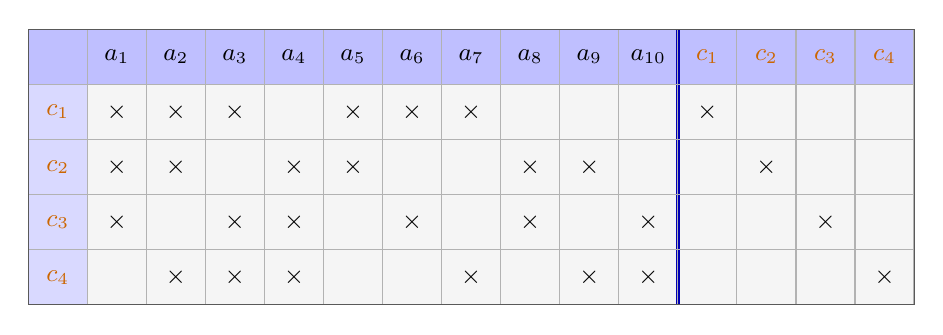
\begin{tikzpicture}[
                x=0.75cm,
                y=0.7cm,
                every node/.style={font=\small}
            ]

            % Hintergrund
            \fill[blue!25] (0,0) rectangle (15,1);
            \fill[blue!15] (0,-4) rectangle (1,0);
            \fill[gray!8] (1,-4) rectangle (15,0);


            % Spaltenbeschriftungen: Nachrichtenbits
            \foreach \i in {1,...,10} {
                    \node at (\i+0.5,0.5) {\(a_{\i}\)};
                }

            % Spaltenbeschriftungen: Kontrollbits
            \foreach \i in {1,...,4} {
                    \pgfmathtruncatemacro{\col}{10+\i}
                    \node[text=orange!80!black]
                    at (\col+0.5,0.5) {\(c_{\i}\)};
                }

            % Zeilenbeschriftungen
            \foreach \i in {1,...,4} {
                    \node[text=orange!80!black]
                    at (0.5,0.5-\i) {\(c_{\i}\)};
                }

            % Überwachungsbereich c1
            \foreach \col in {1,2,3,5,6,7,11} {
                    \node at (\col+0.5,-0.5) {\(\times\)};
                }

            % Überwachungsbereich c2
            \foreach \col in {1,2,4,5,8,9,12} {
                    \node at (\col+0.5,-1.5) {\(\times\)};
                }

            % Überwachungsbereich c3
            \foreach \col in {1,3,4,6,8,10,13} {
                    \node at (\col+0.5,-2.5) {\(\times\)};
                }

            % Überwachungsbereich c4
            \foreach \col in {2,3,4,7,9,10,14} {
                    \node at (\col+0.5,-3.5) {\(\times\)};
                }



            % Trennung Nachrichtenbits / Kontrollbits
            \draw[blue!70!black,very thick] (11,-4) -- (11,1);

            % Gitter
            \draw[step=1,black!30,thin]
            (0,-4) grid (15,1);

            % Äusserer Rahmen
            \draw[black!65]
            (0,-4) rectangle (15,1);

        \end{tikzpicture}
    \end{center}

    \begin{enumerate}
        \item Alice möchte die Nachricht
              \texttt{0101 0101 01} versenden.
              Wie lautet die Nachricht samt Kontrollbits?

        \item Bob erhält die Nachricht
              \texttt{1111 1111 11}
              \textcolor{magenta}{\texttt{1001}}.
              Wie lautet die ursprüngliche Nachricht,
              wenn man davon ausgeht, dass bei der
              Übermittlung höchstens ein Fehler
              passiert ist?

        \item Cedric erhält die Nachricht
              \texttt{1010 1010 11}
              \textcolor{magenta}{\texttt{0111}}.
              Wo ist der Fehler passiert?
    \end{enumerate}

    \begin{myanswer}
        \begin{enumerate}
            \item Die von Alice versendete Nachricht lautet:
                  \[
                      \texttt{0101 0101 01}\,
                      \textcolor{orange}{\texttt{0101}}
                  \]

            \item Die von Bob erhaltene Nachricht hat einen Fehler
                  beim Bit \(a_7\). Ursprünglich lautete die Nachricht:
                  \[
                      \texttt{1111 1101 11}
                  \]

            \item Bei der Nachricht, die Cedric erhält, ist der Fehler
                  im letzten Kontrollbit \(c_4\) passiert.
                  Das korrekte Codewort lautet:
                  \[
                      \texttt{1010 1010 11}\,
                      \textcolor{orange}{\texttt{0110}}
                  \]
        \end{enumerate}
    \end{myanswer}

\end{myexercise}



\begin{myexercise}
    Alice möchte eine 1-fehlerkorrigierende Kodierung für
    8 verschiedene Nachrichten entwerfen. Für die Kodierung
    dieser Nachrichten (ohne Kontrollbits) verwendet sie
    Bitfolgen der Länge 3
    (\texttt{000}, \texttt{001}, \ldots, \texttt{111}).

    \begin{enumerate}
        \item Wie viele Kontrollbits sind für eine
              1-fehlerkorrigierende Kodierung mindestens notwendig?

        \item Entwerfen Sie eine solche Kodierung, indem Sie
              die entsprechende Überwachungstabelle angeben.
    \end{enumerate}
    \begin{myanswer}

        Die Anzahl \(n\) der Kontrollbits muss so gross sein, dass
        \[
            2^n-1 \geq 3+n
        \]
        gilt. Daraus folgt \(n\geq 3\). Es werden also mindestens
        drei Kontrollbits benötigt.

        Eine mögliche Überwachungstabelle ist:

        \begin{center}
            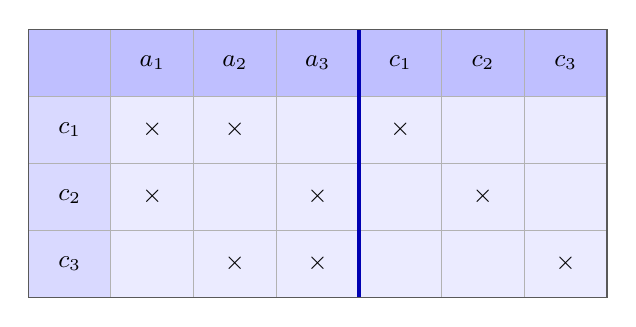
\begin{tikzpicture}[
                    x=1.05cm,
                    y=0.85cm,
                    every node/.style={font=\small}
                ]


                % Hintergrund
                \fill[blue!25] (0,0) rectangle (7,1);
                \fill[blue!15] (0,-3) rectangle (1,0);
                \fill[blue!8] (1,-3) rectangle (7,0);

                % Spaltenbeschriftungen
                \foreach \i in {1,...,3} {
                        \node at (\i+0.5,0.5) {\(a_{\i}\)};
                    }
                \foreach \i in {1,...,3} {
                        \pgfmathtruncatemacro{\col}{3+\i}
                        \node at (\col+0.5,0.5) {\(c_{\i}\)};
                    }

                % Zeilenbeschriftungen
                \foreach \i in {1,...,3} {
                        \node at (0.5,0.5-\i) {\(c_{\i}\)};
                    }

                % Überwachungsbereich c1
                \foreach \col in {1,2,4} {
                        \node at (\col+0.5,-0.5) {\(\times\)};
                    }

                % Überwachungsbereich c2
                \foreach \col in {1,3,5} {
                        \node at (\col+0.5,-1.5) {\(\times\)};
                    }

                % Überwachungsbereich c3
                \foreach \col in {2,3,6} {
                        \node at (\col+0.5,-2.5) {\(\times\)};
                    }

                % Gitter
                \draw[step=1,black!30,thin] (0,-3) grid (7,1);

                % Trennung Nachrichtenbits / Kontrollbits
                \draw[blue!70!black,very thick] (4,-3) -- (4,1);


                % Äusserer Rahmen
                \draw[black!65]
                (0,-3) rectangle (7,1);

            \end{tikzpicture}
        \end{center}

        Die Spalten der Überwachungstabelle sind paarweise verschieden
        und keine Spalte ist leer. Damit kann jeder einzelne Bitfehler
        eindeutig lokalisiert und korrigiert werden.

    \end{myanswer}
\end{myexercise}


\begin{myexercise}
    Bob benötigt eine 1-fehlerkorrigierende Kodierung
    für eine Million verschiedene Nachrichten.

    \begin{enumerate}
        \item Wie viele Bits sind für die Kodierung der
              Nachrichten nötig (ohne Kontrollbits)?

        \item Wie viele Kontrollbits werden mindestens benötigt?
    \end{enumerate}
    \begin{myanswer}
        Für eine Million verschiedene Nachrichten sind Bitfolgen der
        Länge 20 nötig, denn es gilt
        \[
            2^{19} < 10^6 < 2^{20}.
        \]

        Die Anzahl \(n\) der Kontrollbits muss so gross sein, dass
        \[
            2^n-1 \geq 20+n
        \]
        gilt. Für \(n=4\) ist diese Bedingung nicht erfüllt, für
        \(n=5\) hingegen schon:
        \[
            2^5-1=31\geq 25.
        \]

        Es werden also mindestens \textbf{5 Kontrollbits} benötigt.
    \end{myanswer}
\end{myexercise}


\begin{myexercise}

    Entwerfen Sie eine 1-fehlerkorrigierende Kodierung für
    30 verschiedene Nachrichten. Geben Sie die entsprechende
    Überwachungstabelle an.
    \begin{myanswer}

        Für 30 verschiedene Nachrichten benötigt man Bitfolgen der Länge 5,
        da \(2^4 < 30 \leq 2^5\) gilt.

        Für die Anzahl \(n\) der Kontrollbits muss gelten:
        \[
            2^n-1 \geq 5+n.
        \]
        Daraus folgt \(n\geq 4\). Es werden also mindestens
        vier Kontrollbits benötigt.

        Eine mögliche Überwachungstabelle ist:

        \begin{center}
            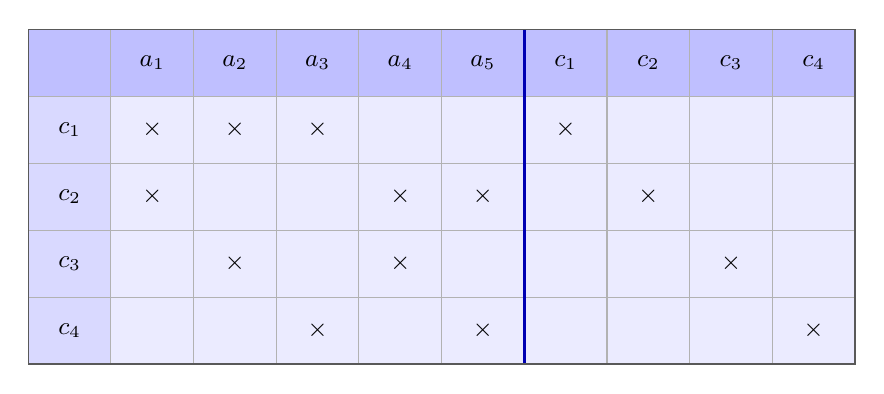
\begin{tikzpicture}[
                    x=1.05cm,
                    y=0.85cm,
                    every node/.style={font=\small}
                ]


                % Hintergrund
                \fill[blue!25] (0,0) rectangle (10,1);
                \fill[blue!15] (0,-4) rectangle (1,0);
                \fill[blue!8] (1,-4) rectangle (10,0);

                % Spaltenbeschriftungen: Nachrichtenbits
                \foreach \i in {1,...,5} {
                        \node at (\i+0.5,0.5) {\(a_{\i}\)};
                    }

                % Spaltenbeschriftungen: Kontrollbits
                \foreach \i in {1,...,4} {
                        \pgfmathtruncatemacro{\col}{5+\i}
                        \node at (\col+0.5,0.5) {\(c_{\i}\)};
                    }

                % Zeilenbeschriftungen
                \foreach \i in {1,...,4} {
                        \node at (0.5,0.5-\i) {\(c_{\i}\)};
                    }

                % Überwachungsbereich c1
                \foreach \col in {1,2,3,6} {
                        \node at (\col+0.5,-0.5) {\(\times\)};
                    }

                % Überwachungsbereich c2
                \foreach \col in {1,4,5,7} {
                        \node at (\col+0.5,-1.5) {\(\times\)};
                    }

                % Überwachungsbereich c3
                \foreach \col in {2,4,8} {
                        \node at (\col+0.5,-2.5) {\(\times\)};
                    }

                % Überwachungsbereich c4
                \foreach \col in {3,5,9} {
                        \node at (\col+0.5,-3.5) {\(\times\)};
                    }

                % Gitter
                \draw[step=1,black!30,thin] (0,-4) grid (10,1);

                % Trennung Nachrichtenbits / Kontrollbits
                \draw[blue!70!black,very thick] (6,-4) -- (6,1);


                % Äusserer Rahmen
                \draw[black!65]
                (0,-4) rectangle (10,1);


            \end{tikzpicture}
        \end{center}

        Da alle Spalten der Überwachungstabelle paarweise verschieden
        und nicht leer sind, kann jeder einzelne Bitfehler eindeutig
        lokalisiert und korrigiert werden.

    \end{myanswer}
\end{myexercise}










\subsection*{Historischer Hintergrund: Richard Hamming}

Die Entwicklung effizienter fehlerkorrigierender Codes ist
eng mit dem amerikanischen Mathematiker Richard Hamming
(1915--1998) verbunden.

Hamming arbeitete zunächst am Manhattan-Projekt und später
bei den Bell Laboratories. Zu dieser Zeit wurden Programme
und Daten unter anderem mithilfe von Lochkarten gespeichert
und eingegeben. Ein Loch entsprach dabei einer 1, eine Stelle
ohne Loch einer 0.

\begin{figure}[H]
    \centering
    \includegraphics[width = 0.5\textwidth]{Grundlagen_Info/05_Datenintegritaet/Figures/Fortran_punch_card_ESA.jpg}
    \caption{Fortran Lochkarte der European Space Agency (ESA), 70er Jahre, Till Niermann, CC BY-SA 3.0, via Wikimedia Commons}
    \label{fig:lochkarte}
\end{figure}

Fehler beim Erstellen oder Lesen der Lochkarten konnten dazu
führen, dass Programme nicht korrekt ausgeführt wurden.
Besonders ärgerlich war, dass solche Fehler oft erst nach
längerer Rechenzeit bemerkt wurden.

Hamming beschäftigte sich deshalb mit der Frage, wie sich
solche Fehler automatisch erkennen und korrigieren lassen.
Daraus entstanden die nach ihm benannten \emph{Hamming-Codes},
die mit vergleichsweise wenigen Kontrollbits einzelne
Bitfehler korrigieren können.

Die Grundidee entspricht dem Verfahren, das wir gerade
untersucht haben: Jedes Bit wird durch eine bestimmte
Kombination von Kontrollbits überwacht. Aus den verletzten
Paritätsbedingungen lässt sich die Position eines einzelnen
fehlerhaften Bits bestimmen.

Damit bilden die Hamming-Codes eine wichtige Grundlage
der Fehlerkorrektur in digitalen Informationssystemen.

\begin{myexercise}
    Mit unseren Überlegungen konnten wir die minimale Anzahl
    Kontrollbits für eine 1-fehler-korrigierende Kodierung ermitteln.
    Bei der Erstellung der entsprechenden Überwachungstabellen
    haben wir viele Freiheiten. Entscheidend ist lediglich, dass
    alle Spalten paarweise verschieden sind und keine Spalte leer ist.

    Richard Hamming entwickelte eine elegante Methode, mit der
    sich systematisch festlegen lässt, welche Bits von den einzelnen
    Kontrollbits überwacht werden und an welchen Positionen die
    Kontrollbits innerhalb des Codeworts stehen sollen. Schliesslich
    müssen die Kontrollbits nicht zwingend am Ende der Nachricht
    angefügt werden.

    Weitere Informationen zur Funktionsweise der Hamming-Codes
    finden Sie im folgenden Video:

    \begin{center}
        \url{https://www.youtube.com/watch?v=X8jsijhllIA}
    \end{center}



    \begin{enumerate}
        \item Alice möchte den \((15,11)\)-Hamming-Code verwenden,
              um die Nachricht \texttt{1011 1100 010} zu versenden.
              Wie lautet die um die Kontrollbits ergänzte Nachricht?

        \item Bob erhält die mit dem \((15,11)\)-Hamming-Code
              kodierte Nachricht \texttt{0001 1011 0010 0011}.
              Korrigieren Sie den Fehler in der Nachricht.
    \end{enumerate}

    \begin{myanswer}

        \begin{enumerate}
            \item Die von Alice versendete Nachricht lautet:
                  \[
                      \texttt{1011 1011 1110 0001}
                  \]

                  \begin{center}
                      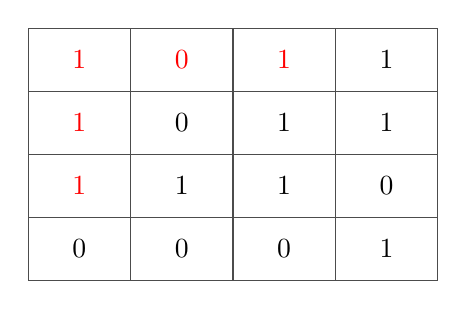
\begin{tikzpicture}[
                              x=1.3cm, y=0.8cm,
                              every node/.style={font=\normalsize}
                          ]
                          \foreach \row/\col/\bit in {
                                  1/1/1, 1/2/0, 1/3/1, 1/4/1,
                                  2/1/1, 2/2/0, 2/3/1, 2/4/1,
                                  3/1/1, 3/2/1, 3/3/1, 3/4/0,
                                  4/1/0, 4/2/0, 4/3/0, 4/4/1
                              } {
                                  \node at (\col-.5,4.5-\row) {\bit};
                              }

                          % Kontrollbits rot hervorheben
                          \foreach \col/\row/\bit in {
                                  1/1/1, 2/1/0, 3/1/1,
                                  1/2/1, 1/3/1
                              } {
                                  \node[red,fill=white,inner sep=1pt]
                                  at (\col-.5,4.5-\row) {\bit};
                              }

                          \draw[step=1,black!70] (0,0) grid (4,4);
                      \end{tikzpicture}
                  \end{center}

            \item Die von Bob erhaltene Nachricht enthält einen
                  Fehler an der Position 14. Das entsprechende Bit
                  muss von 0 auf 1 korrigiert werden.

                  \begin{center}
                      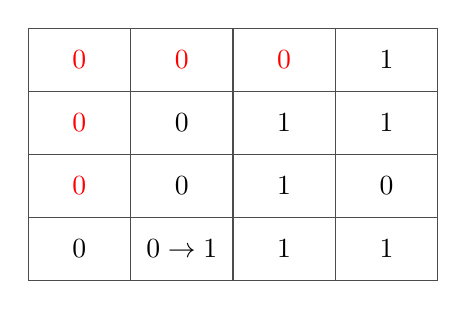
\begin{tikzpicture}[
                              x=1.3cm, y=0.8cm,
                              every node/.style={font=\normalsize}
                          ]
                          \foreach \row/\col/\bit in {
                                  1/1/0, 1/2/0, 1/3/0, 1/4/1,
                                  2/1/1, 2/2/0, 2/3/1, 2/4/1,
                                  3/1/0, 3/2/0, 3/3/1, 3/4/0,
                                  4/1/0, 4/2/0, 4/3/1, 4/4/1
                              } {
                                  \node at (\col-.5,4.5-\row) {\bit};
                              }
                          % Kontrollbits rot hervorheben
                          \foreach \col/\row in {
                                  1/1, 2/1, 3/1, 1/2, 1/3
                              } {
                                  \node[red,fill=white,inner sep=1pt]
                                  at (\col-.5,4.5-\row) {0};
                              }

                          % Fehlerkorrektur an Position 14
                          \node[fill=white,inner sep=1pt]
                          at (1.5,.5)
                          {\(\cancel{0}\rightarrow 1\)};

                          \draw[step=1,black!70] (0,0) grid (4,4);
                      \end{tikzpicture}
                  \end{center}
        \end{enumerate}

    \end{myanswer}

\end{myexercise}









